\chapter{Definizione di un sistema di Enterprise Search per le Risorse Umane}

Lo studio condotto sui temi di Information Retrieval ha trovato finalizzazione nello sviluppo di un motore di ricerca che potesse integrare il proprio funzionamento all’interno di un prodotto aziendale già ben funzionante ed utilizzato. Lo stage di durata trimestrale si è svolto presso l’azienda Capitolo Quinto srl~\footnote{\url{http://www.capitoloquinto.com/}} e il software oggetto del mio studio è Arkivium Recruiting\footnote{\url{http://www.arkivium.com/}}, un applicativo di natura gestionale che rientra nella categoria di \textit{Customer Relationship Management} (CRM). Più specificatamente, il software si occupa della gestione del processo di ricerca e selezione del personale e assume il ruolo di \textit{Applicant Tracking System} (ATS), indicato per il settore delle risorse umane.

Il lavoro di progettazione e realizzazione del sistema è stato condotto con una metodologia di sviluppo incrementale, che a partire dall’analisi delle esigenze è stato in grado di produrre di volta in volta dei risultati intermedi, che affrontassero e risolvessero i problemi riscontrati in maniera evolutiva. È seguendo questo tipo di approccio che vorrei accompagnare il lettore attraverso l’intero processo decisionale che ha dato luce ad un prototipo del motore di ricerca, il quale sarà soggetto nei mesi seguenti ad ulteriori miglioramenti che si concluderanno con il rilascio del prodotto sul mercato.




\section{Analisi dei requisiti}

Arkivium Recruiting è utilizzato da diversi tipi di organizzazioni (agenzie per il lavoro, società di ricerca e selezione, reparti aziendali delle risorse umane) per coordinare e agevolare i processi di ricerca e selezione del personale. Il sistema gestisce numerosi dati, tipici di questo ambito, che vedono la “figura professionale” al centro dell’attenzione, con le proprie competenze ed esperienze pregresse che la rendono parte di una rete costituita da numerose aziende, persone ed enti di formazione. Tali informazioni possono essere a disposizione dei \textit{recruiter} in forma strutturata o, come molto più spesso accade in questo mondo, nascondersi all’interno del \textit{curriculum vitae} di una persona insieme ad una miriade di informazioni che di volta in volta devono essere manualmente consultate ed interpretate dai selezionatori.

In questo contesto nasce l’esigenza di poter effettuare delle ricerche in maniera molto efficiente all’interno di informazioni solo parzialmente strutturate, che provengono in parte da un database ed in parte dai diversi tipi di file associati ad una persona o azienda, fra cui appunto i \textit{curriculum vitae}.

Tale esigenza era in Arkivium già in parte soddisfatta dal precedente motore di ricerca, implementato con Apache Lucene, che permetteva di effettuare ricerche \textit{full text} abbastanza basilari. La necessità di sottoporre interrogazioni più intuitive e di presentare risultati di maggiore utilità per l’utente, nonché di contare su di un sistema maggiormente scalabile, ha inevitabilmente richiesto il passaggio da Lucene a qualcosa di più versatile e facilmente utilizzabile. La scelta è ricaduta su Apache Solr, in grado di offrire numerose opportunità ad elevate prestazioni senza la necessità di stravolgere in alcun modo l’ecosistema nel quale Arkivium abitualmente opera.

\vspace{1em}

Nello specifico, quest’ultimo consiste di un’applicazione web realizzata attraverso il paradigma MVC del Microsoft .NET Framework\footnote{\url{https://www.microsoft.com/net/apps/web}}, all’interno della quale si è inserito il codice per la gestione delle informazioni da indicizzare ed il loro reperimento in fase di ricerca; a tal proposito, per l’utilizzo di Solr si sono utilizzate direttamente le Web API esposte dal server.




\section{Costruzione dell'archivio documentale}

Il primo quesito da affrontare, quando si progetta un motore di ricerca, è \textbf{ciò che si vuole cercare}. Una prima soluzione a cui si potrebbe pensare consiste nella volontà di cercare fin da subito nella totalità delle fonti d’informazione a propria disposizione; tuttavia, dal momento che si ha a che fare con molti dati dai significati più disparati, questo tipo di approccio non è immediato e non è scontato possa rivelarsi una soluzione adatta, perché ciascuna informazione deve influire in maniera adeguata sui risultati della ricerca e deve successivamente essere presentata all’utente nel modo corretto.

Nel caso in esame, i dati trattati dall’applicazione sono vari e tipici di un \textit{Customer Relationship Management}. Non tutti sono oggetto di questo studio, che si concentra solamente sui pilastri fondamentali attorno ai quali è costruita l’intera base informativa: \textbf{Persone}, \textbf{Aziende}, \textbf{Progetti} e \textbf{Documenti}. L’obiettivo è quello di costruire un motore di ricerca in grado di cercare contemporaneamente documenti che rappresentano molteplici tipi di informazioni, senza che l’utente si accorga di alcuna limitazione tecnica che possa derivarne ed in modo che i risultati gli vengano presentati in maniera intuitiva e funzionale.

\vspace{1em}

Il principale sistema di memorizzazione di Arkivium è un database di tipo relazionale, che sfrutta numerose tabelle e associazioni per rappresentare le informazioni a disposizione dei \textit{recruiter}. Le principali entità coinvolte sono \texttt{Persone} e \texttt{Aziende}, a propria volta legate a molteplici \texttt{Progetti}. Ciascun elemento può essere inoltre collegato ad uno o più \texttt{Documenti}, veri e propri file salvati su memoria di massa e il cui riferimento lo si ottiene consultando il database stesso (\texttt{NOTA}: d’ora in poi, il tipo di entità del database che rappresenta un file sarà sempre scritta come \texttt{Documento}, per evitare si possa confondere con il concetto di “documento Solr” precedentemente descritto, che invece rappresenta la metodologia di rappresentazione delle informazioni in Solr).

\vspace{1em}

Affinché le informazioni strutturate presenti nel database (\texttt{Persone}, \texttt{Aziende} e \texttt{Progetti}) e quelle non strutturate costituite dai file (\texttt{Documenti}) possano essere gestite tramite Solr, è necessario convertirle in un formato a questo comprensibile; ciascuna entità deve essere adeguatamente rimodellata sfruttando le informazioni presenti nel database, spesso attingendo a molteplici tabelle o al file system.

Prima di modellare le conoscenze a disposizione partendo dallo schema \textit{Entity-Relationship} che rappresenta il database, è necessario decidere in che modo si vogliono utilizzare gli indici Solr per memorizzare e reperire i documenti a disposizione.



\subsection{Utilizzo degli indici}

Lavorando con Solr, e più precisamente con Lucene che ne sta alla base, è fondamentale decidere in che modo le informazioni devono essere suddivise e memorizzate negli opportuni indici. I fattori da tenere in considerazione sono:

\begin{itemize}
\item necessità informative, in particolare ciò che si vuole ottenere da una singola query;
\item accessibilità delle informazioni, cioè chi deve avere accesso ai dati degli indici.
\end{itemize}


\subsubsection{Suddivisione delle informazioni}

Il precedente motore di ricerca integrato in Arkivium sfruttava due indici, di cui uno per indicizzare le \texttt{Persone} e uno per i \texttt{Documenti}. Questa soluzione prevedeva la necessità di effettuare operazioni differenti sui due, in particolare per quanto riguarda il processo di interrogazione, che poteva agire solamente su un indice per volta con la necessità di sottoporre due query distinte nel caso in cui si volesse ottenere un risultato misto.

Progettando il nuovo sistema ci si è accorti che il modello multi-indice non fosse particolarmente comodo e, in funzione delle necessità informative dell’utente - che potrebbe avere la necessità di cercare, con una singola query, sull’intero contenuto indicizzato -, si è deciso di optare per una soluzione a singolo indice. La natura malleabile di un JSON e quindi di un documento Solr consentono infatti di rappresentare oggetti ben distinti all’interno del medesimo indice, offrendo la possibilità di sfruttare proprietà comuni a più di un oggetto pur personalizzando ciascuno di essi con campi specifici. Esemplificando, è chiaro che una \texttt{Persona} e un \texttt{Documento} siano entrambi caratterizzati da un \textit{nome}, ma il primo abbia bisogno di memorizzare anche una \textit{data di nascita} mentre del secondo si predilige salvare l’\textit{estensione}.

Questo tipo di approccio consente una gestione semplificata dell’intero processo di indicizzazione e ricerca, ma costringe ad aggiungere per ciascun documento un campo che ne identifichi il \textit{tipo}.


\subsubsection{Gestione degli accessi}

La seconda considerazione cui si è andati incontro durante il processo di progettazione è legata alla separazione degli accessi fra clienti. Per “cliente” si intende l’azienda che acquista Arkivium per la gestione dei propri processi di ricerca e selezione. É chiaro che ogni cliente detiene un database con i propri dati ed è essenziale che questi rimangano di natura confidenziale.

Anche questa volta, grazie all’adattabilità di un documento Solr, sarebbe possibile decidere di mettere a disposizione un singolo indice per tutti i clienti di Capitolo Quinto. Ciò prevedrebbe l’inserimento di un ulteriore campo che, per ogni documento, identifichi il cliente a cui appartiene. In fase di interrogazione, l’applicazione dovrebbe fare in modo che ogni cliente possa accedere solamente ai propri dati.

Nonostante la soluzione sia attuabile, è inevitabilmente poco sicura se non adeguatamente gestita, perché potrebbe facilmente portare ad accidentali falle di sicurezza che causerebbero una spiacevole diffusione di informazioni private. Inoltre, così facendo l’indice risultante assumerebbe dimensioni considerevoli e potrebbe essere causa di complicazioni sia a livello prestazionale sia nel caso si presenti la necessità di ricostruire l’indice, un processo di cui si parlerà nella sezione~\ref{sec:indexing} dedicata all’indicizzazione.


\subsubsection{Soluzione adottata}

Ricapitolando, si è scelto di sfruttare un singolo indice per ciascuna azienda che utilizza Arkivium. Ciò consente di soddisfare contemporaneamente i requisiti utente e la necessità di interfacciarsi facilmente con un sistema sicuro. In Solr, ogni indice corrisponde a un \textit{core} del server (o \textit{collection}, se si sta utilizzando SolrCloud), che è caratterizzato da un proprio schema e risponde ad un certo \textit{url}. Ogni cliente utilizzerà l’\textit{url} dedicatogli, il cui accesso in futuro potrebbe essere protetto da autenticazione.



\subsection{Dal modello Entity-Relationship al documento JSON}
\label{sec:modelling}

Riprendendo quanto detto poc’anzi, Arkivium memorizza gran parte delle proprie informazioni all’interno di un database relazionale, che consente di trattare dati ben strutturati e interconnessi. Affinché possano essere utilizzati da Solr, devono essere convertiti in un formato che quest’ultimo sia in grado di interpretare: CSV, XML o JSON. Per semplicità e leggibilità si è scelto di usare il JSON, che consente una modellazione intuitiva e, per certi versi, anche più adatta rispetto ad un approccio relazionale: alcune relazioni \texttt{N:N} sono infatti più facilmente rappresentabili con un JSON piuttosto che tramite il formato tabellare di un database SQL.

Gli elementi più importanti che fanno parte della base di dati informativa di Arkivium sono rappresentati nella figura~\ref{fig:ermodel}, che è solamente un piccolo estratto del complesso diagramma ER che descrive il database. Pur essendo focalizzato solamente sulle tabelle principali \texttt{Person}, \texttt{Company}, \texttt{Attachment} e \texttt{Project} (in azzurro nel modello), lo schema concettuale appare piuttosto intricato a causa delle numerose relazioni che intercorrono fra le diverse entità.

\vspace{1em}
\begin{figure}[H]
	\centering
	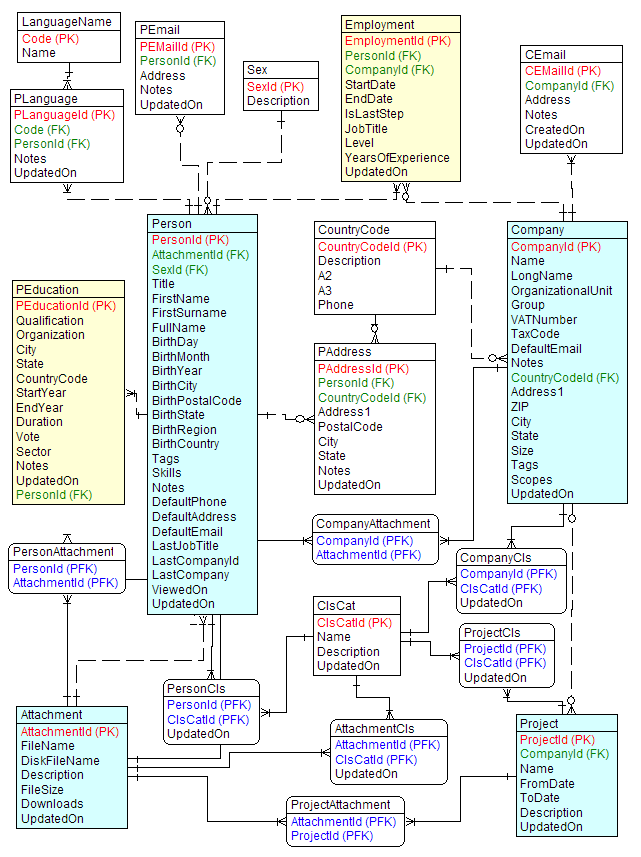
\includegraphics[scale=1]{../images/03_1_ER_v2}
	\caption[Modello ER semplificato del database di Arkivium]{Modello ER del database di Arkivium}
	\label{fig:ermodel}
\end{figure}

\vspace{2em}
\pagebreak

Nel modellare le tabelle in formato JSON sono state effettuate delle scelte atte a descrivere opportunamente le entità coinvolte agendo sulla struttura dei documenti che rappresentano ciascuna tabella, ognuna delle quali caratterizzata da molteplici campi personalizzati. Tutti i documenti dispongono di alcuni campi comuni, necessari per identificarli e descriverli brevemente; quest’ultimi campi costituiscono la struttura di un \textbf{documento base}:
\begin{itemize}
\item \texttt{doc\_type}, un campo \textit{enum} che identifica il \textit{tipo} del documento (e.g, \texttt{Persona}, \texttt{Azienda}, \texttt{Progetto} o \texttt{Documento}).
\item \texttt{arkivium\_id}, che corrisponde all’\textit{id} originale del \textit{record} nel database di Arkivium.
\item \texttt{id}, un campo speciale che Solr utilizza per identificare univocamente i propri documenti all’interno del \textit{core} di appartenenza (questo capo è fondamentale perché usato anche per gestire l’aggiornamento dei documenti in fasi successive alla costruzione dell’indice); nel nostro specifico caso sarà costituito da una stringa, formata dalla concatenazione dei campi \texttt{doc\_type} e \texttt{arkivium\_id}.
\item \texttt{heading}, un campo di tipo testuale, calcolato da Arkivium tramite concatenazione di molteplici informazioni, atto a rappresentare sinteticamente un documento; dovrebbe permettere all’utente di distinguere facilmente un documento dagli altri.
\end{itemize}

Se quelli appena descritti sono i campi che accumunano tutti i documenti da indicizzare, di seguito vengono sinteticamente esposte le caratteristiche specifiche di ogni tipologia di documento. La spiegazione è corredata di eventuali scelte e tecniche utilizzate per la modellazione, facendo sempre riferimento allo schema ER del database nonché tenendo in considerazione i requisiti di ricerca e aggiornamento dei documenti nell’indice. Quanto viene mostrato è il risultato della sequenza di modifiche apportate di volta in volta nel corso della progettazione funzionale del sistema.


\subsubsection{Persone}

Dal modello ER in figura~\ref{fig:ermodel} si evince che per ogni \texttt{Persona} vengono registrati i dati anagrafici (\texttt{Person}) e di contatto (\texttt{PAddress} e \texttt{PEmail}), le lingue conosciute (\texttt{PLanguage}), il sesso (\texttt{Sex}), le classificazioni (\texttt{PersonCls}), le esperienze lavorative (\texttt{PEmployment}) e la formazione (\texttt{PEducation}). Quest’ultime due (in giallo nello schema~\ref{fig:ermodel}) sono descritte da numerosi campi, motivo per cui si è deciso di modellarle come \textit{nested documents}. Ciò significa che \texttt{PEmployment} e \texttt{PEducation} diventeranno dei documenti JSON veri e propri, innestati all’interno del documento padre di \textit{tipo} \texttt{Person}. Ogni \texttt{Esperienza lavorativa} è a propria volta connessa con un’\texttt{Azienda} e tale relazione viene opportunamente memorizzata all’interno del campo \texttt{relations}.

Le restanti proprietà, più semplici, verranno totalmente accorpate all’interno del JSON che rappresenta una \texttt{Persona}, in forma di stringhe, numeri oppure come array. Per finire, si noti che ciascuna \texttt{Persona} può essere connessa ad un arbitrario numero di \texttt{Documenti}, relazione che sarà modellata solamente nel documento di tipo \texttt{Attachment}, per motivi spiegati in seguito. 

\begin{listing}[H]
\begin{minted}{json}
{ 
    "id": "person-15341",
    "doc_type": "person",
    "arkivium_id": 15341, 
    "name": "Ferri Marco",
    "heading": "Ferri Marco Full Stack .NET Developer Capitolo Quinto",
    "location": "Viale Giotto, 1 21052 Busto Arsizio  (VA)  - Italia ",
    "default_email": "96marco@libero.it",
    "last_job_title": "Full Stack .NET Developer",
    "last_company": "Capitolo Quinto",
    "skills": [ "Programming", "Web Development", "ASP.NET MVC" ],
    "classifications": [ "Clienti", "Fornitori" ],
    "_childDocuments_": [
      {
        "start_year": 2015,
        "end_year": 2018,
        "sector": "Informatica",
        "title": "Laurea Triennale - Informatica",
        "organization": "Universita' degli Studi di Milano-Bicocca",
        "relations": [ "person-15341" ],
        "doc_type": "education",
        "arkivium_id": 87,
        "id": "education-87",
        "updated_on": "2018-05-14T10:48:54.4127Z"
      },
      {
        "start_date": "2016-07-01T00:00:00Z",
        "title": "Full Stack .NET Developer",
        "organization": "Capitolo Quinto",
        "location": "via Italia, 10 - 20121 Milano  (MI)  - Italia ",
        "relations": [ "person-15341", "company-16289" ],
        "doc_type": "employment",
        "arkivium_id": 16394,
        "id": "employment-16394",
        "heading": "Full Stack .NET Developer Capitolo Quinto",
        "updated_on": "2018-06-01T09:42:08.6814Z"
      }
    ]
}
\end{minted}
\caption{JSON che rappresenta un documento Solr di tipo \texttt{Persona}}
\label{code:personjson}
\end{listing}

\vspace{-0.5em}
Il codice~\ref{code:personjson} mostra il documento che rappresenta una \texttt{Persona}, dal quale si evince che molte informazioni sono state semplificate e il risultato sia decisamente più leggibile rispetto a quanto possa accadere con un database relazionale. Il campo \texttt{heading} è composto dalla concatenazione dei campi più significativi, \texttt{location} rappresenta sinteticamente le informazioni di un indirizzo e i documenti innestati relativi a \texttt{Educazione} e \texttt{Professione} sono stati rappresentati nell’array \texttt{\_childDocuments\_}. Tale array assume un ruolo speciale in Solr ed è l’unico modo per indicizzare documenti innestati.

\vspace{1em}
Ovviamente la costruzione di un JSON di questo tipo richiede numerose operazioni di \textit{join} sul database durante la fase di indicizzazione di una \texttt{Persona}.


\subsubsection{Aziende e Progetti}

Entrambi condividono i ragionamenti validi per le \texttt{}{Persone}, pertanto non ci si soffermerà ad analizzarli approfonditamente né si mostreranno i corrispettivi documenti in formato JSON. I risultati sono molto semplici: sono state opportunamente modellate solamente le proprietà utili per la ricerca e il campo \texttt{heading} è ancora una volta ottenuto dalla concatenazione dei campi più rappresentativi del documento.


\subsubsection{Documenti}

I \texttt{Documenti} sono rappresentati nel database tramite la tabella \texttt{Attachment}. La modellazione JSON è molto simile alle precedenti, ma ciascun \texttt{Attachment} è dotato del campo \texttt{relations}, un array di stringhe atto a contenere gli \texttt{id} di tutti i documenti con i quali è in relazione, che siano essi \texttt{Persone}, \texttt{Aziende} o \texttt{Progetti}. Un array è il modo migliore per rappresentare l’associazione di tipo \texttt{N:N} fra documenti per mezzo di opportuni \textit{reference} (gli \texttt{id}), che in un contesto relazionale sarebbero rappresentati dalle chiavi esterne. Su questo campo è possibile effettuare opportune \textit{join query}\footnote{\url{https://wiki.apache.org/solr/Join}}.

\vspace{0.5em}
\begin{listing}[H]
\begin{minted}{json}
{
    "id":"attachment-18789",
    "doc_type":"attachment",
    "arkivium_id":18789,
    "heading":"dropbox cover letter.txt",
    "name":"d83e97dd-6b55-45e0-892d-6fdb0dceb361.txt",
    "description":"CV Marco",
    "filename":"dropbox cover letter.txt",
    "extension":"txt",
    "relations":[
      "person-15341",
      "company-12345",
      "project-12344"
    ],
    "classifications":["Curriculum"],
    "updated_on":"2018-05-16T13:10:59Z"
}
\end{minted}
\caption{JSON che rappresenta un documento Solr di tipo \texttt{Documento}}
\label{code:documentjson}
\end{listing}

\vspace{-0.5em}
Rappresentare le relazioni \textbf{solo} nel documento di tipo \texttt{Attachment} (collegandolo a \texttt{Person/Company}/\texttt{Project}), evitando la rappresentazione speculare da \texttt{Person}/\texttt{Company}/ \texttt{Project} ad \texttt{Attachment}, è una scelta atta ad ottimizzare l’indicizzazione \textit{real time}. La pratica verrà spiegata in seguito, nella sezione~\ref{sec:realtimeindexing}; per ora è sufficiente ragionare sul fatto che l’aggiornamento (o inserimento) di un \texttt{Attachment} nel database di Arkivium avviene in concomitanza all’assegnazione dello stesso ad una o più \texttt{Persone/Aziende/Progetti}. È normale quindi che la modifica di un \texttt{Attachment} porti con sé le relazioni ad esso associate, senza però intaccare nessuna delle altre tabelle. Alla luce di questa considerazione, si rivela triviale aggiornare il campo \texttt{relations} di un \texttt{Attachment} nel momento in cui si modificano le sue relazioni, operazione che non sarebbe altrettanto banale se si dovessero contemporaneamente aggiornare degli ipotetici campi \texttt{attachments} all’interno dei documenti (\texttt{Persone}, \texttt{Aziende} e \texttt{Progetti}) associati all’\texttt{Attachment} stesso.

\vspace{1em}

È importante notare che, nonostante ogni \texttt{Attachment} si riferisca di fatto ad un vero e proprio file su disco, in questa fase della modellazione non si parla ancora del suo contenuto. Sarà in seguito necessario conoscere il \textit{path} di memorizzazione del file, per poterlo recuperare dal file system e inviarlo a Solr affinché Tika ne estragga il contenuto, che sarà quindi indicizzato (ed eventualmente memorizzato) nel campo \texttt{content}.




\subsection{Schema Solr - prima versione}
\label{sec:schema1}

La modellazione dei dati in formato JSON prevede la definizione dei campi atti a contenere le informazioni sulle quali è necessario effettuare le ricerche. Ciascun campo in Solr deve essere \textbf{tipizzato}, in maniera analoga a quanto accade in un linguaggio di programmazione \textit{object-oriented}. Campi e tipi sono descritti all’interno dello \textbf{schema}\footnote{\url{https://lucene.apache.org/solr/guide/7\_4/documents-fields-and-schema-design}}, che definisce quale deve essere la struttura degli indici Lucene sottostanti e come trattare il contenuto di ciascun campo. 

\vspace{1em}

Lo schema viene descritto in XML tramite un apposito file, a scelta fra i seguenti:
\begin{itemize}
\item \texttt{managed-schema}, l’impostazione di default, consente di effettuare modifiche allo schema solo tramite apposite API e permette di usufruire dell’approccio \textit{schemaless};
\item \texttt{schema.xml} è il file tradizionale, che consente solo modifiche manuali.
\end{itemize}

Per il caso in esame si è voluto esercitare un forte controllo sullo schema, motivo per cui è stata accantonata la modalità \textit{schemaless}. Dunque, per comodità di modifica del file si è scelto di utilizzare il file \texttt{schema.xml}.


\pagebreak
\subsubsection{FieldTypes}

All’interno dello schema si definiscono innanzitutto i tipi (\texttt{fieldType}) che verranno utilizzati per la dichiarazione dei campi (\texttt{field}). Ciascun tipo è caratterizzato da un nome univoco e associato ad una classe Java che ne definisce il comportamento primario; successivamente, tramite appositi attributi, si specificano ulteriori proprietà:

\begin{itemize}
\item \texttt{required}, determina se un campo è obbligatorio;
\item \texttt{indexed}, determina se su un campo è concessa la ricerca;
\item \texttt{stored}, determina se il valore del campo è memorizzato e quindi restituito fra i risultati di una query;
\item \texttt{multiValued}, determina se un campo è multivalore;
\item \texttt{docValues}, definisce apposite strutture per ottimizzare alcune interrogazioni.
\end{itemize}

Se il \texttt{fieldType} è di natura testuale è necessario descrivere anche l’\textbf{analisi del testo} prescelta per ciò che esso contiene, costituita innanzitutto da un \texttt{Tokenizer}\footnote{\url{https://lucene.apache.org/solr/guide/7\_4/tokenizers.html}} che si occupa di suddividere il flusso di caratteri in \textit{token}, poi seguito da una catena di \texttt{Filter}\footnote{\url{https://lucene.apache.org/solr/guide/7\_4/filter-descriptions.html}} che analizzano, scartano o trasformano i \textit{token} prima dell’indicizzazione.

\vspace{2em}

La prima versione dello schema pensata per Arkivium nasce senza particolari pretese, per ottenere dei risultati semplici ma efficaci. Lo schema di default, che dichiara i principali tipi Solr, viene leggermente modificato per rimuovere i contenuti superflui e adattarlo alle esigenze dell’applicazione.
Per i campi testuali si è scelto di usare un’analisi molto minimale, mostrata nel seguente listato.

\begin{listing}[H]
\begin{minted}{xml}
<fieldType name="text_general" class="solr.TextField">
  <analyzer type="index">
    <tokenizer class="solr.StandardTokenizerFactory"/>
    <filter class="solr.StopFilterFactory" words="stopwords.txt" ignoreCase="true"/>
    <filter class="solr.LowerCaseFilterFactory"/>
  </analyzer>
  <analyzer type="query">
    <tokenizer class="solr.StandardTokenizerFactory"/>
    <filter class="solr.StopFilterFactory" words="stopwords.txt" ignoreCase="true"/>
    <filter class="solr.SynonymGraphFilter" expand="true" synonyms="synonyms.txt"/>
    <filter class="solr.LowerCaseFilterFactory"/>
  </analyzer>
</fieldType>
\end{minted}
\caption{\texttt{schema.xml} - analisi testuale per i campi di tipo \texttt{text\_general}}
\label{code:schema1texttype}
\end{listing}

\pagebreak
\noindent Tale processo di analisi testuale si occupa di:
\begin{itemize}
\item Suddividere il testo in \textit{token} (\texttt{StandardTokenizerFactory});
\item Rimuovere le \textit{stop word}, contenute nel file \texttt{stopwords.txt} (\texttt{StopFilterFactory});
\item Solo in fase di interrogazione, espandere la query con i sinonimi specificati nel file \texttt{synonyms.txt} (\texttt{SynonymGraphFilterFactory});
\item Convertire i \textit{token} in lettere minuscole (\texttt{LowerCaseFilterFactory}).
\end{itemize}

\vspace{2em}
Successivamente, con l’ausilio del file di configurazione \texttt{enums.xml} mostrato nel listato~\ref{code:schema1enum}, vengono inoltre definiti gli \textit{enum} che descrivono i possibili valori assunti dei campi \texttt{document\_type}, \texttt{project\_type} e \texttt{sex}.

\vspace{0.5em}
\begin{listing}[H]
\begin{minted}{xml}
<enumsConfig>
  <enum name="DocumentType">
    <value>person</value>
    <value>company</value>
    <value>project</value>
    <value>attachment</value>
    <value>education</value>
    <value>employment</value>
  </enum>
  <enum name="ProjectType">
    <value>bip</value>
    <value>mailing</value>
    <value>recruiting</value>
  </enum>
  <enum name="Sex">
    <value>female</value>
    <value>male</value>
  </enum>
</enumsConfig>
\end{minted}
\caption{\texttt{enums.xml} - dichiarazione dei tipi \textit{enum}}
\label{code:schema1enum}
\end{listing}

\vspace{-1em}
\begin{listing}[H]
\begin{minted}{xml}
<fieldType name="document_type" class="solr.EnumFieldType" docValues="true"
            enumsConfig="enums.xml" enumName="DocumentType"/>
            
<fieldType name="project_type" class="solr.EnumFieldType" docValues="true" 
            enumsConfig="enums.xml" enumName="ProjectType"/>
            
<fieldType name="sex" class="solr.EnumFieldType" docValues="true" 
            enumsConfig="enums.xml" enumName="Sex"/>
\end{minted}
\caption{\texttt{schema.xml} - utilizzo di campi \textit{enum}}
\label{code:schema1enumuse}
\end{listing}

\subsubsection{Fields}

Definiti i \texttt{fieldType}, si procede ad elencare i campi che costituiranno la struttura dei documenti da indicizzare.

\vspace{1em}
\begin{listing}[H]
\begin{minted}{xml}
<uniqueKey>id</uniqueKey>
<field name="id" type="string" required="true" />
<field name="doc_type" type="document_type" required="true" />
<field name="arkivium_id" type="pint" />
<field name="heading" type="text_general" />
<field name="updated_on" type="pdate" />
\end{minted}
\caption{\texttt{schema.xml} - campi comuni a tutti i documenti}
\label{code:schema1field1}
\end{listing}
\vspace{-1em}
I campi comuni a tutti i \textit{tipi} di documento vengono dichiarati per primi. Dall’XML del listato~\ref{code:schema1field1} si evince che il campo \texttt{id} serve a identificare univocamente un documento (\texttt{uniqueKey}) e, come \texttt{doc\_type}, è obbligatorio. \texttt{Heading} è un campo di \textit{testo}, mentre \texttt{arkivium\_id} e \texttt{updated\_on} sono rispettivamente puntatori a un \textit{intero} e a una \textit{data}.

\vspace{1.8em}
\begin{listing}[H]
\begin{minted}{xml}
<field name="name" type="text_general" />
<field name="description" type="text_general" />
<field name="notes" type="text_general" />
<field name="location" type="text_general" />
<field name="default_email" type="string" />
<field name="relations" type="strings" />
\end{minted}
\caption{\texttt{schema.xml} - alcuni campi specifici di alcuni \textit{tipi} di documento}
\label{code:schema1field2}
\end{listing}
\vspace{-1em}

Successivamente si definiscono tutti gli altri campi, che per brevità non sono qui interamente elencati. Da questo piccolo campione emerge \texttt{default\_email}, che è del tipo \textit{stringa} e cioè, nonostante di natura testuale, trattato come se il suo contenuto costituisse un unico termine. Anche \texttt{relations} è dello stesso tipo, ma \textit{multivalore}.

\vspace{1.8em}
\begin{listing}[H]
\begin{minted}{xml}
<field name="_text_" type="text_general" multiValued="true" stored="false"/>
<copyField source="name" dest="_text_" />
<copyField source="description" dest="_text_" />
<copyField source="notes" dest="_text_" />
<copyField source="location" dest="_text_" />
<copyField source="default_email" dest="_text_" />
\end{minted}
\caption{\texttt{schema.xml} - altri campi di esempio}
\label{code:schema1field3}
\end{listing}
\vspace{-1em}

Il campo \texttt{\_text\_} è un elemento fondamentale ed assume il cosiddetto ruolo di \textit{catchAll field}, adibito alla raccolta delle informazioni più importanti provenienti dagli altri campi. È utile impostarlo come \texttt{defaultField} di ricerca (nel file \texttt{solrconfig.xml}), affinché una query possa interrogare questo campo per cercare nella totalità delle informazioni a disposizione. Si noti che il suddetto è \texttt{multiValued} ma non memorizzato (\texttt{stored="false"}), poiché ha solo finalità di ricerca e non è necessario che venga restituito fra i risultati di una query. Per creare un campo \textit{catchAll} si fa uso dei \texttt{copyField}\footnote{\url{https://lucene.apache.org/solr/guide/7_4/copying-fields.html}}, che consentono di copiare un campo (\texttt{source}) all’interno di un altro (\texttt{dest}), \textbf{prima} che il suo contenuto venga analizzato.

\vspace{1.8em}
\begin{listing}[H]
\begin{minted}{xml}
<field name="classifications" type="text_general" multiValued="true" />
<copyField source="classifications" dest="classifications_str" />
\end{minted}
\caption{\texttt{schema.xml} - campo \texttt{classifications}}
\label{code:schema1field4}
\end{listing}
\vspace{-1em}

L’ultimo elemento qui presentato è il campo \texttt{classifications}. Raccoglie le informazioni provenienti dalle tabelle \texttt{PersonCls}, \texttt{CompanyCls}, \texttt{ProjectCls} e \texttt{ClsCat} del database, che servono a suddividere i dati in “categorie”. Data la natura e lo scopo di questa categorizzazione, tale campo si presta molto bene ad una \textbf{\textit{faceted search}}, motivo per cui si rivela fondamentale preservare invariato il testo all’interno dell’indice affinché possa essere presentato all’utente nella sua interezza durante il \textit{faceting}, che altrimenti verrebbe suddiviso in \textit{token} e sottoposto alla catena di filtri risultando irriconoscibile per l’utente. È comune, quindi, effettuare una copia dei campi sui quali si hanno questo tipo di esigenze.

\vspace{1em}

Più nello specifico, per effettuare la copia si sfrutta il concetto di \texttt{dynamicField}\footnote{\url{https://lucene.apache.org/solr/guide/7_4/dynamic-fields.html}}, che permette di definire dei tipi di natura dinamica, sfruttando il \textit{suffisso} (o il \textit{prefisso}) del nome di un campo.

\vspace{-0.3em}
\begin{listing}[H]
\begin{minted}{xml}
<dynamicField name="*_str" type="strings" 
		docValues="true" indexed="false" stored="false"/>
\end{minted}
\caption{\texttt{schema.xml} - esempio di \texttt{dynamicField}}
\label{code:schema1field5}
\end{listing}
\vspace{-1em}

Il risultato è che dal campo \texttt{classification} viene creato un nuovo campo di nome \texttt{classification\_str}, non indicizzato, né memorizzato o analizzato (\texttt{strings}), ma ottimizzato per il \textit{faceting} (\texttt{docValues="true"}).




\section{Processo di indicizzazione}
\label{sec:indexing}

La costruzione (\textit{build}) degli indici è il primo problema che si è affrontato durante lo sviluppo del sistema. Il processo ha lo scopo di fornire al server le informazioni da indicizzare ed è fondamentale, poiché durante questa fase che Solr analizza i documenti ricevuti per indicizzarli secondo le modalità descritte nello schema. L’importazione in Solr dell’intera mole di informazioni a disposizione avviene una tantum, durante l’inizializzazione del sistema, e successivamente ogni volta che si ha la necessità di ricostruire gli indici in seguito ad una modifica dello schema che prevede la reindicizzazione dei documenti (\textit{rebuild}).

Qualsiasi successiva modifica, da parte dell’utente, alle informazioni contenute in Arkivium deve essere propagata anche al server Solr affinché le ricerche risultino consistenti. L’operazione di aggiornamento degli indici di Lucene non è banale, ma Solr mette a disposizione specifiche funzionalità per rendere il processo quanto più trasparente ed immediato possibile, affinché l’utente non si accorga di nulla.

\vspace{1em}

Vengono ora descritte le fasi di creazione a aggiornamento degli indici, ponendo particolare attenzione alle metodologie con le quali sono state implementate dall’applicazione. Si presentano alcune strategie risolutive strettamente legate all’ambiente di sviluppo di Arkivium, ma replicabili da qualsiasi ecosistema con simili funzionalità.



\subsection{Esportazione del database}

\textit{Build} e \textit{rebuild} di un indice sono operazioni che possono richiedere molto tempo e capacità computazionali, sia per reperire le informazioni da inviare a Solr sia per quanto riguarda il processo di analisi a cui ciascun documento deve essere sottoposto da parte del server. Si è scelto di gestire questo tipo di operazioni tramite appositi programmi batch, da eseguire all’occorrenza.

\vspace{1em}

Arkivium è sviluppato in ambiente .NET e sfrutta un database relazionale come principale unità di memorizzazione delle informazioni. L’importazione dei dati in Solr ha avuto inizio con l’esportazione del database. A tale scopo si è sfruttato \textit{Entity Framework}\footnote{\url{https://docs.microsoft.com/it-it/ef/}}, il più famoso \textit{Object Relationship Mapping} (ORM) di casa Microsoft, per effettuare le dovute query sul database e reperire tutte le informazioni da inviare a Solr. 

\vspace{1em}

Più nello specifico, partendo dalle tabelle \texttt{Person}, \texttt{Company}, \texttt{Project} e \texttt{Attachment}, viste in figura~\ref{fig:ermodel}, si sono effettuate le opportune operazioni di \textit{join} sul database per ricavare dei \textit{Data Transfer Object} (DTO) atti a rappresentare i documenti prescelti durante la fase di modellazione dei dati; sono state create le classi C\# \texttt{SolrPerson}, \texttt{SolrCompany}, \texttt{SolrProject} e \texttt{SolrAttachment}.

Gli oggetti di tipo \texttt{SolrPerson}, \texttt{SolrCompany} e \texttt{SolrProject} sono stati convertiti in JSON, seguendo le opportune convenzioni Solr, e inviati al server affinché il \textit{request handler}\footnote{\url{https://lucene.apache.org/solr/guide/7_4/uploading-data-with-index-handlers}}  che risponde all’indirizzo \url{\#host\#/update} potesse interpretare i documenti ricevuti e indicizzarli secondo le disposizioni contenute nello schema. \newline
Al contrario, gli \texttt{Attachment} sono stati sottoposti ad una procedura differente poiché differente è il \textit{request handler}\footnote{\url{https://lucene.apache.org/solr/guide/7_4/uploading-data-with-solr-cell-using-apache-tika}} che gestisce l’estrazione del contenuto testuale di un file attraverso Apache Tika (sezione~\ref{sec:solrcell}) e risponde all’indirizzo \url{\#host\#/update/extract}. In questo caso il parametro di input principale è il file stesso, le cui proprietà devono essere elencate non come JSON bensì attraverso la \textit{querystring} della richiesta, serializzando opportunamente la classe \texttt{SolrAttachment}.

\vspace{1em}

A causa dell’elevato numero di \textit{join} sul database e conversioni necessarie per modellare opportunamente ciascun documento, come spiegato nella sezione~\ref{sec:modelling}, ogni esecuzione del processo batch di esportazione richiede un quantitativo di risorse non indifferente e può impiegare anche diverse ore per essere portato a termine. Allo stesso modo, anche l’importazione dei dati in Solr è soggetta ad una richiesta di risorse non indifferente, tanto più alta quanto più complicata è l’analisi testuale cui si sottopone ciascun documento. Per questi motivi è bene che le operazioni di \textit{rebuild} siano effettuate solo quando strettamente necessario e preferibilmente durante periodi in cui l’utilizzo del sistema sia minimo (ad esempio di notte o nel weekend), affinché l’utente non si accorga di eventuali rallentamenti.



\subsection{Dimensioni degli indici}

La dimensione degli indici dipende dal quantitativo di documenti indicizzati, dal numero dei termini che entrano a far parte del dizionario dell'indice e dalla quantità di testo che si decide di memorizzare per ciascun documento (attributo \texttt{stored}). Inoltre, le dimensioni sono soggette a periodici cambiamenti causati dalla gestione a basso livello degli indici. Nello specifico, Solr deve occuparsi di rendere disponibili per la ricerca le informazioni indicizzate come se facessero parte di un unico indice, quando nella realtà è consuetudine avere a che fare con molteplici indici che attendono di essere sottoposti ad un \textit{merge}. Tale operazione viene eseguita durante l’ottimizzazione di un \textit{core} (o \textit{collection}) e richiede un elevato numero di risorse; è da eseguirsi periodicamente, durante momenti di minimo utilizzo del sistema, e può causare un aumento temporaneo delle dimensioni degli indici.

\vspace{1em}

In funzione di queste considerazioni non è possibile fornire una stima precisa della crescita di un indice Solr. Per quanto riguarda i test effettuati durante questa prima fase dello sviluppo si è riscontrato che, sfruttando un’analisi testuale molto basica come quella prescelta per il primo schema (descritto nella sezione~\ref{sec:schema1}), le dimensioni degli indici sono davvero ridotte. Nello specifico, indicizzare circa 65mila documenti ha richiesto solamente uno spazio di circa \textbf{100 MB}\footnote{Un test con circa 1 milione di documenti ha prodotto un indice dalla dimensione di 1,5 GB}, considerando che l’unica informazione non memorizzata (\texttt{not stored}, non reperibile fra i risultati di una query) si trattava del contenuto estratto dai file, esclusivamente indicizzato, nel campo \texttt{content}.

Si mostrerà in seguito che la memorizzazione di \texttt{content}, nonché un’analisi testuale decisamente più complessa atta a migliorare il \textit{matching} fra query e documenti, farà aumentare considerevolmente la dimensione degli indici. Per lo stesso numero di documenti saranno necessari ben \textbf{10 GB} di indici \textbf{non ottimizzati}.



\pagebreak
\subsection{Near real time search}
\label{sec:realtimeindexing}

Quando un utente inserisce o aggiorna un dato appartenente al database di Arkivium è necessario che tale modifica venga propagata al server Solr affinché le informazioni ricercabili rimangano coerenti. I due sistemi infatti, nonostante siano progettati per cooperare, esistono indipendentemente l’uno dall’altro ed è premura del programmatore fare in modo che rimangano allineati.

A questo scopo si è deciso di implementare tramite \textit{Entity Framework} (EF) un meccanismo che invii al server Solr un documento ogni qualvolta viene effettuata la modifica di una tabella del database sulla quale si hanno esigenze di ricerca. In breve, con EF ciascuna tabella del database è modellata per mezzo di una classe C\#, di cui un’istanza rappresenta un \textit{record} della tabella stessa. Per aggiornare o inserire un nuovo \textit{record} nel database è sufficiente istanziare un oggetto e indicare al framework che lo si vuole salvare nel database; un apposito metodo (\texttt{SaveChanges}) si occuperà di gestire il salvataggio. È possibile ridefinire il metodo di salvataggio affinché esegua operazioni personalizzate, ed è questa la strategia che si è rivelata fondamentale per aggiornare il server Solr ogni qualvolta se ne rilevi il bisogno. Più dettagliatamente, si è creata un’interfaccia C\# con il solo scopo di contrassegnare le classi indicizzabili; tale interfaccia è quindi stata implementata dalle classi \texttt{Person}, \texttt{Company}, \texttt{Project} e \texttt{Attachment}, affinché durante l’esecuzione del metodo \texttt{saveChanges} ci si potesse accorgere della necessità di indicizzare questo tipo di oggetti e, di conseguenza, serializzarli per l’invio al server Solr. Tale procedura è opportunamente configurata per le operazioni \texttt{INSERT}, \texttt{UPDATE} e \texttt{DELETE} sul database.

\vspace{1em}

Questa soluzione è risultata molto innovativa rispetto a quella adottata dal precedente sistema di ricerca implementato in Lucene. Infatti, come precedentemente accennato, ogni modifica ad un indice implica la creazione di strutture temporanee le cui informazioni possono essere rese visibili per la ricerca solo in un secondo momento. Per questo motivo, utilizzando Lucene diventa necessario programmare l’aggiornamento e il \textit{merge} degli indici con cadenza periodica; nel caso di Arkivium, questi venivano aggiornati tutte le notti e ciò stava a significare che un utente era in grado di cercare nuove informazioni solo il giorno seguente il loro inserimento.

Con Solr questo problema è quasi totalmente superato, poiché introduce funzionalità di ricerca e indicizzazione \textit{near real time}\footnote{\url{https://lucene.apache.org/solr/guide/7_4/near-real-time-searching.html}}. Ciò significa che, nonostante la gestione degli indici rimanga affidata a Lucene, la piattaforma mette a disposizione alcune operazioni che coinvolgono log, memoria volatile e memoria stabile in maniera assolutamente trasparente per l’utente e per il programmatore, rendendo possibile la visualizzazione delle modifiche in tempi relativamente brevi.

\pagebreak
\noindent Si introducono i concetti di:
\begin{itemize}
\item \textit{soft commit}, che rende visibili i cambiamenti pur lasciandoli su memoria volatile;
\item \textit{(hard) commit}, che salva le ultime modifiche su memoria stabile;
\item \textit{optimize}, che effettua il \textit{merge} dei vari segmenti costituenti l’indice.
\end{itemize}
Le tre operazioni hanno costi importanti, sia computazionali che di spazio, ed è opportuno che vengano utilizzate con cognizione di causa, specie in un ambiente soggetto a frequenti aggiornamenti. È possibile configurare la frequenza con la quale devono essere eseguiti \textit{soft commit} e \textit{hard commit}. 

Non c’è una regola precisa per pianificare l'esecuzione dei comandi, ma personalmente consiglio un \textit{soft commit} ogni 10-240 secondi, in base alle esigenze informative dell’utente e il carico di lavoro al quale il server Solr è sottoposto. Gli \textit{hard commit} trasferiscono a tutti gli effetti le nuove informazioni su memoria stabile e prevengono perdite di dati dovute ad eventuali crash del software, ma sono più costosi ed è per questo motivo che potrebbero bastare un paio di esecuzioni all’ora. È comunque consigliato disattivare entrambe le funzioni durante \textit{build} e \textit{rebuild} dell’indice.

Infine, \textit{optimize} è un processo decisamente più oneroso che può richiedere anche molte ore per essere portato a termine; pertanto se ne consiglia un utilizzo periodico, con cadenza giornaliera o settimanale, per ottimizzare considerevolmente la gestione dello spazio su disco ed eventualmente agevolare le prestazioni di ricerca.




\section{Interfaccia di ricerca}

L’interfaccia utente è parte fondamentale della realizzazione di un motore di ricerca, specie in un contesto di \textit{enterprise search} che, a differenza della classica \textit{web search}, prevede l’utilizzo di numerose funzionalità e parametri di ricerca altamente specializzati. Come per il resto del sistema, anche lo sviluppo della GUI ha seguito un approccio di sviluppo incrementale ed è forse questa la fase in cui si evince maggiormente l’evoluzione graduale del motore di ricerca.



\subsection{Progettazione dell’esperienza utente}

Esigenze informative e intuitività di utilizzo sono i punti cardine che hanno condotto la progettazione del sistema dal punto di vista utente, che usufruisce dell’applicazione attraverso il proprio \textit{web browser}.

\vspace{1em}

Il precedente sistema integrato in Arkivium consentiva di effettuare delle ricerche focalizzate solamente su \texttt{Persone} e \texttt{Documenti}, prevedendo un approccio di ricerca \textit{bottom-up}: per sottoporre le richieste, l'utente era costretto a recarsi nelle apposite pagine e comporre la propria query indicando il testo da cercare attraverso multipli input testuali, ognuno dei quali corrispondente a un campo dell’indice Lucene sottostante.

Nonostante tale soluzione si riveli in molti casi adatta alle esigenze informative di un \textit{recruiter}, si è pensato che questo tipo di \textit{workflow} potesse rivelarsi tutto sommato abbastanza limitante. È per questo motivo che riprogettando l’esperienza utente si è pensato di affrontare le ricerche con una metodologia \textit{top-down}: predisporre una barra di ricerca principale \textbf{sempre accessibile} all’utente, qualunque sia l’operazione che si sta svolgendo, che sia in grado di \textbf{cercare su tutte le informazioni a disposizione}, e cioè sul fatidico campo \texttt{\_text\_} che è stato introdotto nello schema (listato~\ref{code:schema1field2}). L’interfaccia che presenta il risultato di questa generica interrogazione dovrebbe quindi ben suddividere le informazioni reperite affinché l’utente riesca immediatamente a discriminare il \textit{tipo} dei documenti trovati. A questo punto sarà possibile raffinare ulteriormente la ricerca con apposite funzioni.

\vspace{1em}

Ciascuna delle funzionalità avanzate è stata introdotta gradualmente all’interno dell’interfaccia, nell’ottica di un miglioramento incrementale non invasivo e costantemente intuitivo per l’utente, che dovrebbe essere in grado di utilizzare il motore di ricerca senza che vi sia la necessità di una particolare esperienza o formazione pregressa.



\subsection{Invio di richieste e interpretazione dei risultati}

Nonostante questo capitolo sia principalmente dedicato ad elementi di usabilità del software, è opportuno specificare che ogni funzione messa a disposizione dell’utente, semplice o complessa che si riveli, è il risultato di uno sviluppo a 360 gradi: studio teorico della funzionalità, codifica della richiesta, \textit{parsing} dei risultati e realizzazione dell’interfaccia grafica che consenta all’utente di sottoporre la query e visualizzarne i risultati in maniera opportuna.

\vspace{1em}

Il paradigma MVC ha consentito un’adeguata separazione delle responsabilità. La pagina dei risultati (la \textit{view}) è sempre renderizzata dal web server (quindi dal \textit{controller}) e l’utilizzo di Javascript è stato ridotto al minimo. Il front-end è stato progettato affinché ciascuna modifica dei parametri di ricerca provochi un \textit{refresh} della pagina, che passa il controllo al back-end e nello specifico a un \texttt{client} .NET creato \textit{ad hoc} per comunicare con Solr e soddisfare la richiesta espressa nella \textit{querystring} (che costituisce il \textit{model}). Tale \texttt{client} interpreta il \textit{model} e invia l’opportuna richiesta HTTP al server Solr, attende il risultato e ne effettua il \textit{parsing}. Infine lo restituisce al \textit{controller}, il quale renderizza la \textit{view} da inviare al browser dell’utente, che finalmente può consultare i risultati della propria query.

Dal momento in cui viene sottoposta richiesta, l’applicazione è in grado di presentare un risultato strutturato all’utente in meno di un secondo. L’effettiva esecuzione della query sul server Solr impiega un tempo molto ridotto rispetto a quanto richiesto invece dalla renderizzazione della \textit{view} da parte del \textit{controller}, che costituisce la fase computazionalmente più dispendiosa a causa della numerosità degli elementi da visualizzare adeguatamente in pagina a seguito dell’interpretazione della risposta ricevuta dal server. In futuro si potrebbe pensare di implementare il processo esecutivo tramite AJAX per ridurre ulteriormente i tempi di attesa e migliorare l’esperienza utente.



\subsection{Interrogazioni di base}

La possibilità di poter effettuare una ricerca in qualsiasi istante è stato il primo obiettivo che ci si è posti per lo sviluppo e ha dato inizio alla realizzazione dell’interfaccia grafica. A tale scopo si è optato per una soluzione molto classica che ha visto l’introduzione di una casella di testo nella parte superiore di tutte le pagine dell’applicazione. È stata concepita affinché la ricerca di una o più parole attraverso la stessa provochi sempre l’apertura di una \textit{nuova scheda del browser}, affinché l’utente, quando si accorge dell’esigenza di cercare qualcosa, non debba interrompere bruscamente l’operazione in corso di svolgimento.

\vspace{1em}

Si è tentato di approcciare questo tipo di ricerca tenendo in considerazione le aspettative dell’utente nei confronti di una barra di ricerca globale, che per tradizione sul Web ha lo scopo di cercare quanto richiesto nella totalità della mole di informazioni disponibili, discriminando opportunamente la rilevanza dei contenuti sui quali viene effettuata la ricerca. Se ad esempio l’utente sta cercando un nome di persona, è naturale che fra i risultati della ricerca appaiano ben in evidenza le persone con tale nome, mentre minore importanza venga riservata, per esempio, ai \textit{curriculum} nei quali il nome è presente ma compare sotto una voce meno significativa, come può essere l’elenco dei correlatori di una tesi di laurea.

Tale esigenza può essere soddisfatta con Lucene assegnando un peso a ciascuna delle parole o dei campi sui quali si sta effettuando la ricerca. Tale pratica prende il nome di \textbf{boosting} e prevede che la query venga formulata con una specifica sintassi\footnote{\url{https://lucene.apache.org/core/2\_9\_4/queryparsersyntax.html\#Boosting\%20a\%20Term}}, non particolarmente complicata ma sicuramente poco intuitiva da ricordare da parte di un utente. Progettando una soluzione che si rivelasse trasparente per l’utente, si è scoperto che Solr mette a disposizione nuovi parametri e sintassi per la composizione delle query, tramite l’utilizzo di opportuni \textit{query parser}.

%\vspace{1em}

Fra questi, particolarmente utile è stato il \textit{query parser} \texttt{edismax}\footnote{\url{https://lucene.apache.org/solr/guide/7_4/the-extended-dismax-query-parser.html}}, che si dimostra più tollerante agli errori sintattici e aggiunge nuove funzionalità al \textit{parser} standard di Lucene. Fra queste, vi è l’introduzione del parametro \textit{query field} (\texttt{qf}), attraverso il quale è possibile elencare i campi dei documenti sui quali deve essere effettuata la ricerca, permettendo inoltre di specificare dei \textit{boost} su ciascuno di essi. \newline
Si è quindi scelto di utilizzare \texttt{edismax} come \textit{parser} di tutte le ricerche e insieme ad esso si è stabilito un insieme di parametri comuni a ciascuna richiesta, affinché l’utente possa sempre beneficiare di alcune comodità che verranno di volta in volta introdotte durante tutto lo sviluppo del motore di ricerca. La barra di ricerca finora descritta costituirà sempre la query principale, e cioè il parametro \texttt{q} di una richiesta.

\vspace{1em}

La prima pagina realizzata per la visualizzazione dei risultati di una ricerca è davvero molto basilare e la si può osservare in figura~\ref{fig:gui1}. Consiste in una semplice tabella che elenca i documenti reperiti dall’esecuzione della query, suddivisi per pagine ma poco interpretabili da parte dell’utente. In questa fase dello sviluppo, le uniche personalizzazioni consentite sono la scelta del numero di documenti da visualizzare per ciascuna pagina e la possibilità di decidere se l’insieme delle parole inserite nell’apposita \textit{}{search bar} siano da cercare in \texttt{AND} (tutte devono essere presenti nei documenti affinché vengano considerati rilevanti) oppure in \texttt{OR} (è sufficiente che i documenti contengano almeno una delle parole cercate).

\begin{figure}[H]
	\centering
	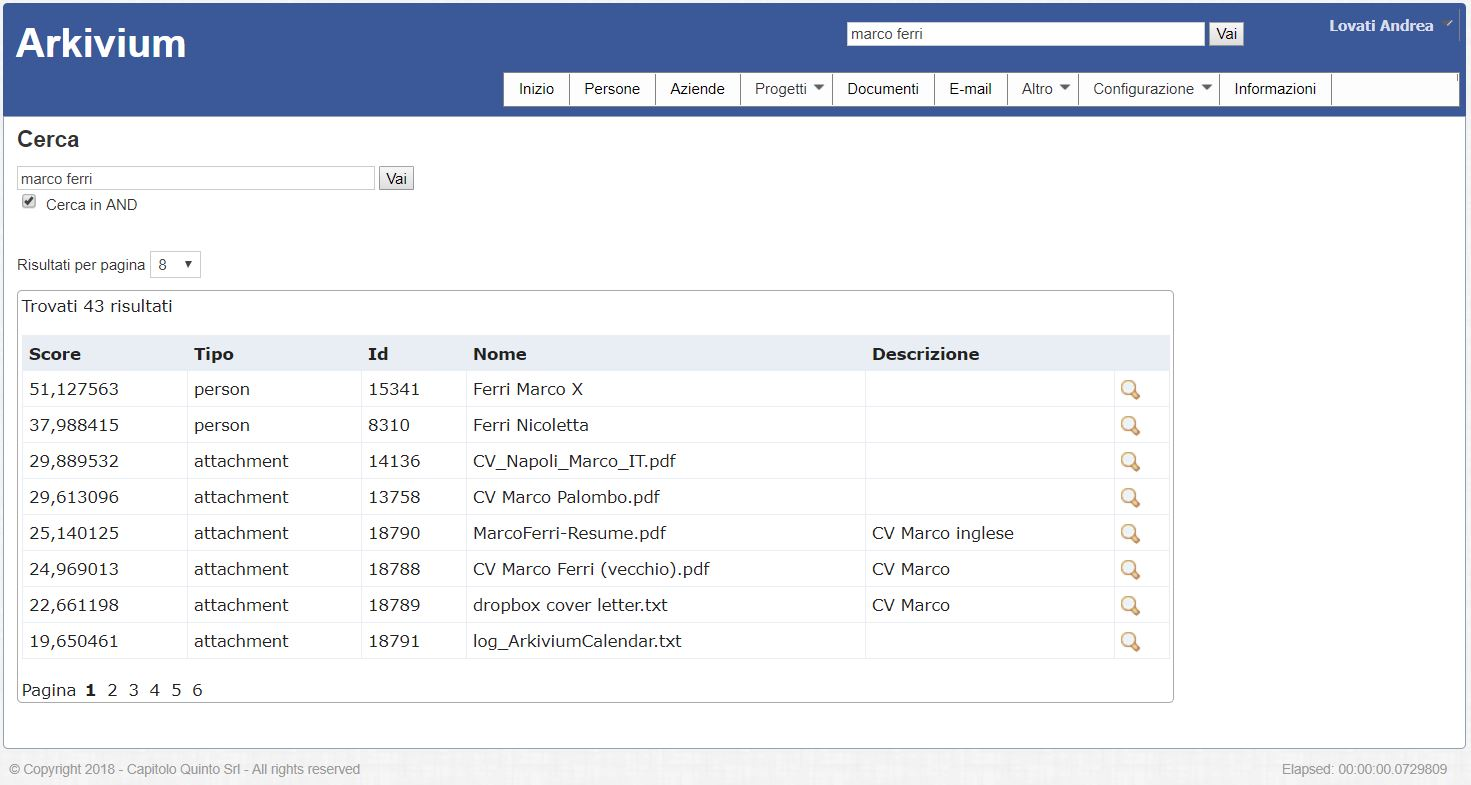
\includegraphics[scale=0.50]{../images/03_2_gui_v1}
	\caption[Prima versione della nuova pagina di ricerca pensata per Arkivium]{Prima versione della nuova pagina di ricerca pensata per Arkivium}
	\label{fig:gui1}
\end{figure}

Con così poche informazioni non si è tuttavia in grado di discriminare immediatamente né il tipo di documento cui ciascuna riga appartiene, né il motivo per cui esso sia stato stimato come rilevante da parte del sistema. Tale pagina è stata sottoposta a miglioramenti graduali atti ad ampliarne usabilità e funzionalità.


\subsection{Faceted search}

Per consentire una maggiore leggibilità dei risultati di ricerca ed in particolare comprendere immediatamente la natura delle informazioni trovate, si è deciso di realizzare un’interfaccia che presenti i documenti reperiti suddivisi per \textit{tipo}: \texttt{Persone}, \texttt{Aziende}, \texttt{Progetti} e \texttt{Documenti}. Questo approccio consente inoltre di personalizzare il modo in cui viene visualizzato ciascun \textit{tipo} di documento, progettando un meccanismo che permetta all’utente di passare da una visualizzazione all’altra, ciascuna delle quali è stata implementata tramite un apposito \textit{tab}.

\vspace{1em}

È importante che l’utente sia consapevole del numero di documenti reperiti per ciascun \textit{tipo}, affinché possa opportunamente decidere su cosa concentrare la propria attenzione. Ciò si concretizza nell’implementazione di una ricerca “sfaccettata”\footnote{\url{https://lucene.apache.org/solr/guide/7_4/faceting.html}}, che consente di ottenere il conteggio dei documenti (fra quelli reperiti) che assumono specifici valori per un determinato campo.

Se il campo su cui si effettua il \textit{faceting} è il \texttt{doc\_type}, si ottengono le informazioni necessarie ad associare il conteggio a ciascun \textit{tab}. La scelta di un \textit{tab} da parte dell’utente determina il \textit{tipo} dei documenti attraverso cui filtrare la query, per mezzo del parametro \textit{filter query} (\texttt{fq}). Il filtro è stato implementato in modo che la scelta di un \textit{tab} non influisca sul conteggio dei documenti appartenenti ad altri \textit{tab} (cioè ad un \textit{tipo} diverso da quello prescelto dall'utente); tale conteggio risulterebbe altrimenti sempre \texttt{0}, dato che l’appartenenza di un documento ad un certo \textit{tipo} esclude l’appartenenza agli altri.

È stato anche predisposto un \textit{tab Generale} che consenta la visualizzazione dei documenti reperiti indipendentemente dal \textit{tipo}. É doveroso inoltre far notare che \texttt{Formazione} ed \texttt{Esperienze professionali}, nonostante siano informazioni innestate all’interno di una \texttt{Persona}, vengono trattati da Solr come se fossero documenti veri e propri e di conseguenza sono stati dedicati loro appositi \textit{tab}. \newline
Nella figura~\ref{fig:gui2} viene mostrato il risultato.

\vspace{2em}

Applicando il \textit{faceting} ad altri campi è possibile ottenere un’ulteriore suddivisione dei documenti in “categorie”, che possono essere sfruttate per raffinare il risultato della ricerca. La funzionalità è stata implementata per default in tutte le richieste, solamente sui campi che assumono valori prestabiliti o circoscritti in un dominio ristretto. Il risultato consiste in gruppi di \textit{checkbox}, uno per campo, che hanno preso posto sulla zona destra dell’interfaccia e consentono di filtrare la query principale.

\begin{figure}[H]
	\centering
	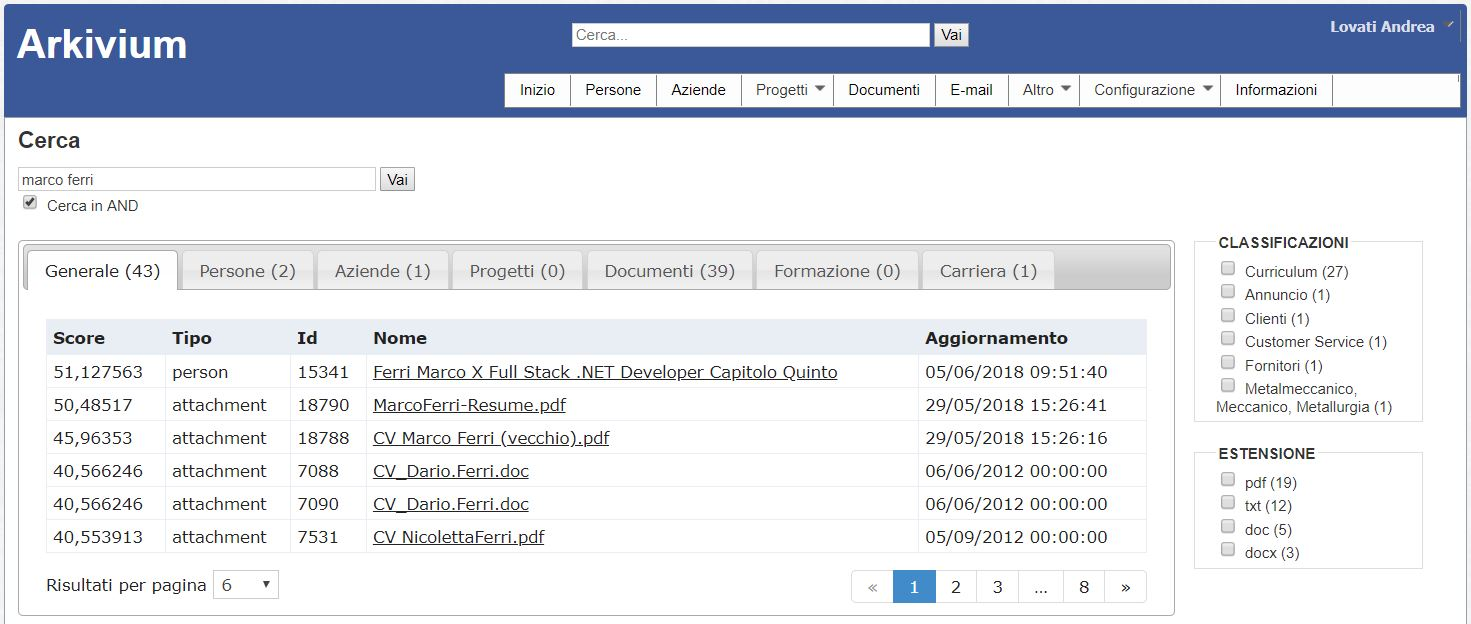
\includegraphics[scale=0.5]{../images/03_3_faceting}
	\caption[Implementazione grafica del \textit{faceting}]{Implementazione grafica  del \textit{faceting}}
	\label{fig:gui2}
\end{figure}



\subsection{Ricerca e ordinamento per campo}

Nonostante - se correttamente implementata - una ricerca globale sia in grado di produrre ottimi risultati, in un contesto come quello delle risorse umane può rivelarsi necessario sottoporre delle query più strutturate per filtrare i documenti con una maggiore precisione. È per questo motivo che vengono introdotte le interrogazioni e l’ordinamento \textit{per field}, che consentono di avere un maggiore controllo dei risultati.

In base ai campi che si vogliono interrogare, la ricerca può essere testuale oppure focalizzata su tipi di dati numerici, temporali, geografici o enumerativi; è compito dell’applicazione mettere a disposizione i componenti grafici adatti a sottoporre richieste che siano coerenti rispetto ai campi da interrogare.

\vspace{1em}

Nel corso dello studio ci si è focalizzati principalmente sui campi di testo, ma come si può osservare in figura~\ref{fig:gui3} sono stati effettuati dei test anche su range numerici (\texttt{anno}) ed \textit{enum} (\texttt{sesso}). Ciascun \textit{tab} è stato dotato degli appositi filtri ed è stata introdotta la possibilità di ordinare i risultati per campo, oltre che per rilevanza.

Le ricerche per campo sono state implementate attraverso il parametro \textit{filter query} (\texttt{fq}), che applica una selezione preventiva sull’indice prima di effettuare la query primaria (parametro \texttt{q}): ciò significa che i \textit{filter query} non hanno alcuna influenza sul punteggio (\texttt{score}) dei documenti e quindi sul concetto di rilevanza.

\begin{figure}[H]
	\centering
	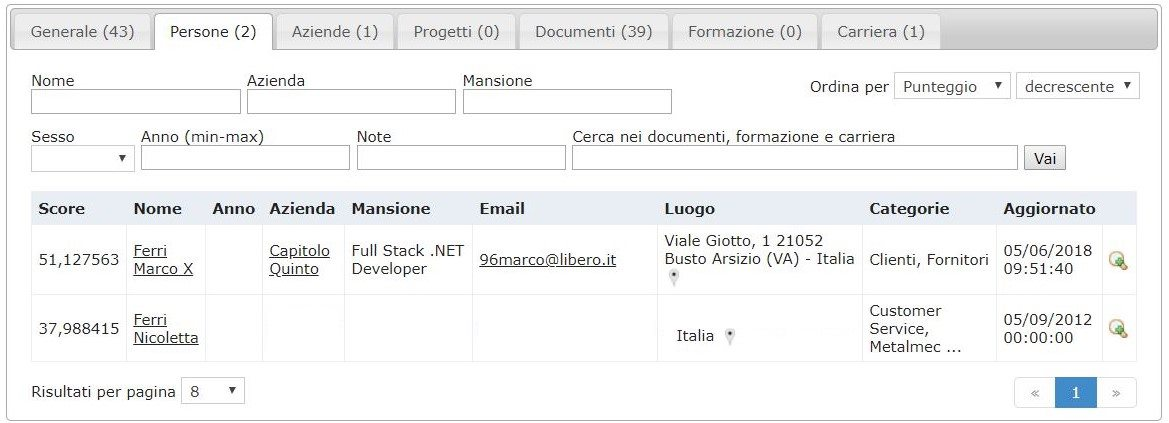
\includegraphics[scale=0.63]{../images/03_4_per_field_search}
	\caption[Esempio di ricerche e ordinamento \textit{per field}]{Esempio di ricerche e ordinamento \textit{per field}}
	\label{fig:gui3}
\end{figure}

Fra i filtri caratterizzanti una \texttt{Persona}, è stato inoltre introdotta un’ulteriore casella di testo con la dicitura \textit{“Cerca nei documenti, formazione e carriera”}. Questa costituisce una funzionalità molto importante per il caso di studio in esame, perché attraverso opportune \textit{join query}\footnote{\url{https://wiki.apache.org/solr/Join}} consente di effettuare interrogazioni congiunte all’interno di documenti Solr fra loro in relazione, come quelli che rappresentano \texttt{Persone} e \texttt{Documenti}. In questo modo, l’utente può combinare la ricerca sulle \texttt{Persone} alla ricerca sui \texttt{Documenti} delle persone filtrate, e quindi ad esempio analizzare i \textit{curriculum} in maniera più precisa. È inoltre possibile sfruttare la medesima tecnica anche per cercare nei documenti innestati, come nel caso di \texttt{Formazione} e \texttt{Carriera}.



\subsection{Highlighting}

Gli strumenti che sono finora stati presentati e fanno parte dell’interfaccia utente consentono di effettuare query abbastanza complesse ma efficienti.

\vspace{1em}
Un possibile esempio di query potrebbe essere: 
“Cerca tutte le \texttt{Persone}, ordinate per \texttt{nome}, in cui compaia la parola \textit{developer}, che lavorino in \textit{Google}, abbiano la parola \textit{Java} nel \texttt{curriculum} e abbiano frequentato un \texttt{corso} di \textit{informatica} in \textit{Bicocca}.”
\vspace{0.5em}

\noindent Se la query è così articolata risulta semplice comprendere i motivi che hanno portato un determinato documento a essere considerato rilevante: soddisfa tutte le richieste. 

\vspace{1em}
Viceversa, se la query è espressa più vagamente - come avviene nella maggior parte dei casi - diventa difficile comprendere i motivi che hanno prodotto un determinato risultato. Per questo motivo nasce l’\textbf{\textit{highlighting}}\footnote{\url{https://lucene.apache.org/solr/guide/7_4/highlighting.html}}, una funzione che consente di mettere in evidenza i termini della query che sono stati trovati nei documenti. Ciò si rivela particolarmente utile nel caso in cui si stia effettuando la ricerca su testi molto lunghi, per i quali diventa molto difficile individuare le occorrenze delle parole cercate.

A tal proposito si è deciso di introdurre l’\textit{highlighting} come parametro comune a tutte le richieste, facendolo operare su tutti i campi dei documenti. Affinché funzioni, i campi su cui agisce devono essere indicizzati (\texttt{indexed}) e memorizzati (\texttt{stored}), pertanto si è rivelato necessario modificare lo schema per memorizzare anche il \texttt{content} estratto dai \texttt{Documenti}, precedentemente solo indicizzato. Dopo un processo di \textit{rebuild} si è notato che la dimensione degli indici \textbf{non ottimizzati} è quadruplicata; ciò si rivelerà un elemento critico nella fase di miglioramento dell’analisi testuale.

\begin{figure}[H]
	\centering
	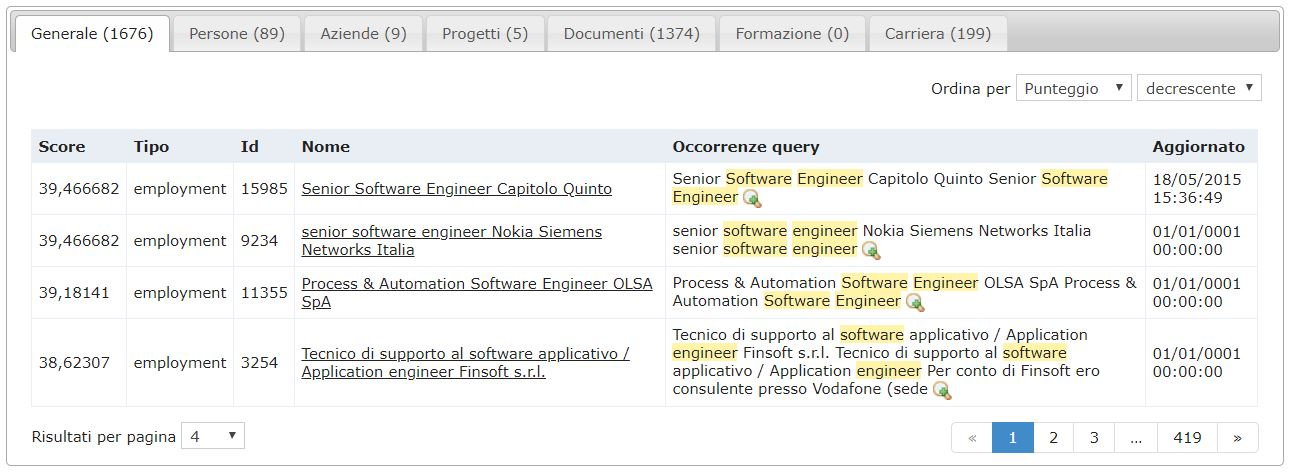
\includegraphics[scale=0.57]{../images/03_5_highlight}
	\caption[Implementazione della funzione di \textit{highlighting}]{Implementazione della funzione di \textit{highlighting}}
	\label{fig:gui4}
\end{figure}



\pagebreak
\subsection{Una nuova \textit{search bar}}

Con Lucene (e Solr) è consentito effettuare ricerche di parole multiple in \texttt{AND} oppure in \texttt{OR}, ma è anche possibile indicare, con un’opportuna sintassi, che si desidera cercare frasi esatte (\textit{\textbf{phrase query}}) o termini simili a quelli indicati nella query (\textit{\textbf{fuzzy query}})\footnote{\url{https://lucene.apache.org/solr/guide/7\_4/the-standard-query-parser.html}}.

\begin{wrapfigure}[9]{r}{6cm}
	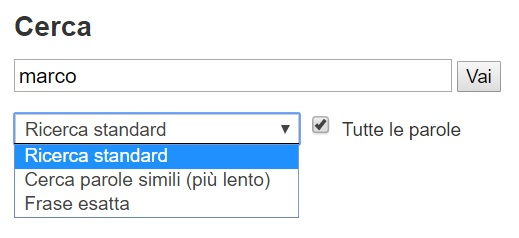
\includegraphics[scale=0.57]{../images/03_6_search_bar}
	\caption[Nuova \textit{search bar}]{Nuova \textit{search bar}}
  	\label{fig:gui5}
\end{wrapfigure}

\vspace{1em}

Questo tipo di ricerche possono rivelarsi utili in determinate situazioni, ma è poco probabile che l’utente medio ricordi le opportune sintassi, che non dovrebbe essere tenuto a conoscere. Si è quindi deciso di rendere trasparenti le funzionalità all’interno dell’interfaccia, riprogettando la barra di ricerca secondo quanto mostrato nella figura ~\ref{fig:gui5}. All’elenco di funzioni mancherebbe la possibilità di specificare le parole che l’utente vuole \textbf{non} compaiano all’interno dei risultati.

\vspace{1em}

Infine, sfruttando il \textit{suggester}\footnote{\url{https://lucene.apache.org/solr/guide/7_4/suggester.html}} di Solr è stato implementato anche l’\textbf{autocompleta-mento} della query attraverso opportuni dizionari, ricavati dai termini memorizzati nell’indice inverso; ciò consente all’utente di essere guidato durante la composizione dell’interrogazione.

In futuro si potrà pensare di sfruttare lo \textit{spellcheck}\footnote{\url{https://lucene.apache.org/solr/guide/7_4/spell-checking.html}}  per implementare il cosiddetto \textit{“forse cercavi...”} o eventualmente correggere (espandere) automaticamente la query dell’utente, in caso di errori di battitura.




\section{Miglioramento dei risultati di ricerca}

L’ultimo problema che si è affrontato riguarda il processo di analisi da operare sul contenuto testuale dei documenti, prima che essi vengano indicizzati, affinché i risultati di un’interrogazione si rivelino davvero utili per le esigenze informative dell’utente. Lo scopo è quello di massimizzare la frazione di documenti rilevanti che vengono reperiti (\textit{richiamo}), minimizzando il reperimento di documenti non rilevanti (\textit{precisione}). Si è deciso di lasciare alla fine la trattazione dell’argomento poiché decisamente complesso e indipendente rispetto alla progettazione dell’interfaccia, che ha richiesto tempistiche di sviluppo importanti.

\vspace{1em}

In prima battuta si è previsto uno schema che proponesse una catena di analisi molto minimale (\textit{tokenization > stop word removing > lowercasing}), completamente indipendente dalla lingua di utilizzo e anche piuttosto limitante. Il meccanismo di \textit{matching} di Lucene si basa sul \textbf{confronto esatto} dei termini ricavati durante le fasi di indicizzazione e interrogazione, quindi è importante che le corrispettive analisi producano termini adeguatamente confrontabili. Se le parole contenute nel testo venissero indicizzate così come sono, l’utente potrebbe avere serie difficoltà nel sottoporre query che reperiscano una buona percentuale di risultati rilevanti rispetto alla totalità dei documenti rilevanti indicizzati (il concetto di \textit{richiamo} enunciato nella sezione \ref{sec:IRSrating}).

\vspace{1em}

L’aspetto principale da considerare durante l’analisi testuale è la \textbf{lingua}: ciascuna possiede regole morfologiche ben precise, pertanto sarebbe opportuno che ogni documento (o campo) venga analizzato per mezzo di operazioni linguistiche altrettanto specifiche.

Ciò non è sufficiente, perché per ottenere un \textit{matching} realmente versatile è necessario trattare adeguatamente tutti i caratteri separatori ed eventualmente consentire anche il \textbf{confronto parziale} fra termini. Se un utente cerca la parola \textit{develop}, tendenzialmente si aspetta che vengano reperiti anche i documenti contenenti la parola \textit{\textbf{develop}er}. Con il meccanismo di \textit{matching} di Lucene questo non avviene e non risulta per niente banale configurare il sistema per ottenere risultati che siano accettabili sia dal punto di vista dell’efficacia (\textit{precisione/richiamo}) che dell’efficienza (\textit{spazio/tempo}).
\newline Questo è un problema ben noto\footnote{Algolia si propone su questo come alternativa a Lucene~\cite{partialmatchingangolia}}, che richiede una considerevole esperienza sul campo ed è stato affrontato con un approccio di tipo sperimentale, atto al raggiungimento di una soluzione qualitativamente accettabile.



\subsection{Ristrutturazione dello schema - seconda versione}

\subsubsection{Analisi linguistica}

L’analisi linguistica è un argomento estremamente complesso, che per essere affrontato nella maniera corretta dovrebbe innanzitutto prevedere un sistema di rilevamento automatico della lingua, affinché si possano successivamente applicare al testo un insieme di operazioni altamente specifiche che consentano di interpretarne correttamente i contenuti e fornire un adeguato supporto alla ricerca.

Le principali operazioni linguistiche consistono nello \textit{stemming}, ossia il “troncamento” di ciascuna parola ad una forma più basilare, e l’espansione dei termini della query attraverso i \textit{quasi-sinonimi}, parole con una forte correlazione semantica rispetto ai termini originali. Entrambi i passaggi sono molto utili affinché ciascuna interrogazione sia sufficientemente versatile: ad esempio, è logico che la ricerca della parola \textit{developer} in una base documentale in lingua italiana dovrebbe reperire anche tutti i documenti nei quali compaiono le parole \textit{programmatore}, \textit{programmatrice}, \textit{sviluppatori}, \textit{software engineer}, etc.

\vspace{1em}

L’implementazione dello \textbf{\textit{stemming}}, in Solr, consiste esclusivamente nella scelta del corretto algoritmo da utilizzare~\cite{elasticstemming} fra i molti a disposizione, motivo per cui appare di fondamentale importanza il processo di rilevamento linguistico cui si accennava poc’anzi. Tuttavia, anche supponendo di essere in grado di discriminare la lingua di un documento (o campo), il processo di rilevamento linguistico non si rivela particolarmente immediato per quanto riguarda la query, che è solitamente composta da un numero di parole decisamente esiguo. É importante che la catena operazionale applicata ai \textit{token} in fase di indicizzazione e interrogazione sia compatibile, pertanto se documenti e query venissero sottoposti a processi linguistici differenti il \textit{matching} ne risulterebbe fortemente alterato.

In funzione di questa considerazione si è deciso, per Arkivium, di omettere ciascun tipo di rilevamento linguistico in favore di una soluzione che potesse rivelarsi adeguata per la maggior parte delle situazioni. In particolare, si è considerato che la stragrande maggioranza dei documenti con cui il software si trova a che fare sono in lingua italiana e inglese, perciò si è pensato di tentare un approccio insolito, di doppia analisi: ciascun termine è stato sottoposto prima allo \textit{stemming} italiano e successivamente a quello inglese, entrambi implementati da algoritmi poco invasivi. Ciò si è tradotto nell’utilizzo di ben 6 \texttt{Filter} consecutivi, mostrati nel blocco di codice~\ref{code:schema2} e successivamente approfonditi. Anche la rimozione delle \textit{stop word} è stata condotta con approccio bi-lingue, raggruppando le parole tipiche dei due linguaggi nel medesimo file di testo.

\vspace{1em}

L’\textbf{espansione dei termini} richiede invece l’utilizzo di opportuni dizionari e tesauri linguistici; nonostante ne esistano alcune versioni pubblicamente disponibili, non sempre si rivelano adatte alle esigenze di ricerca poiché molte relazioni di \textit{quasi-sinonimia} fra termini sono fortemente dipendenti dal contesto applicativo e sarebbe pertanto opportuno che tali risorse venissero costruite \textit{ad hoc} per ciascuna situazione.

Per il caso di studio in esame si è pensato di semplificare il problema, limitandosi ad utilizzare un unico file di testo che sarà adibito a contenere tutti i sinonimi più importanti delle lingue italiano e inglese. In futuro verrà data la possibilità all’utente di inserire nel file i propri sinonimi, affinché l’elenco risulti personalizzato rispetto alle esigenze del contesto nel quale il motore di ricerca deve essere di volta in volta utilizzato.


\subsubsection{Matching parziale dei termini}

Come precedentemente accennato, il \textit{matching} di Lucene si basa sul \textbf{confronto esatto} dei termini. Ciò significa che se per esempio un utente cerca la parola \textit{consulting} nel campo \textit{ragione sociale} di un’\texttt{Azienda}, normalmente non verranno reperite anche le \texttt{Aziende} che si chiamano ad esempio \textit{ConsultingPro}, \textit{srlconsulting} o \textit{12consulting34}. Per risolvere questo problema si è proceduto in due modi.

\vspace{1em}

Innanzitutto si è introdotto un filtro che si occupi di separare i termini che contengono caratteri speciali non trattati dallo \texttt{StandardTokenizer} (ad esempio il punto), lettere maiuscole (notazione \textit{PascalCase}) e numeri. Ciò è implementato in Solr dal \texttt{\textbf{WordDelimiterGraphFilter}}, che si rivela particolarmente utile per la ricerca di indirizzi email, siti web o nomi dei file.

Successivamente si è pensato di abilitare il vero e proprio \textbf{\textit{matching} parziale} attraverso un’ulteriore suddivisione di ciascun \textit{token} in sequenze di caratteri che Solr definisce \textbf{N-Grams} e costituiscono tutte le possibili combinazioni di \textit{prefissi}, \textit{suffissi} e \textit{infissi} del \textit{token} stesso. Tale operazione consente al sistema di \textit{matchare} tutti i termini che \textbf{contengono} una determinata stringa, come avviene per l’operatore \texttt{LIKE} del linguaggio SQL. L’\texttt{NGramFilter}\footnote{\url{https://lucene.apache.org/solr/guide/7_4/filter-descriptions.html\#n-gram-filter}} è da applicare solo in fase di indicizzazione, perché se utilizzato anche durante l’analisi della query è causa di innumerevoli falsi positivi.


\subsubsection{Presentazione del nuovo schema}

La catena di analisi testuale predisposta nella prima versione dello schema Solr, per comodità riportata nel listato~\ref{code:schema1}, è stata completamente rivista per adattarsi alle nuove considerazioni.

\begin{listing}[H]
\begin{minted}
{xml}
<fieldType name="text_general" class="solr.TextField">
  <analyzer type="index">
    <tokenizer class="solr.StandardTokenizerFactory"/>
    <filter class="solr.StopFilterFactory" words="stopwords.txt" ignoreCase="true"/>
    <filter class="solr.LowerCaseFilterFactory"/>
  </analyzer>
  <analyzer type="query">
    <tokenizer class="solr.StandardTokenizerFactory"/>
    <filter class="solr.StopFilterFactory" words="stopwords.txt" ignoreCase="true"/>
    <filter class="solr.SynonymGraphFilter" expand="true" synonyms="synonyms.txt"/>
    <filter class="solr.LowerCaseFilterFactory"/>
  </analyzer>
</fieldType>
\end{minted}
\caption{\texttt{schema.xml} - prima procedura prevista per l'analisi del testo}
\label{code:schema1}
\end{listing}

Il blocco~\ref{code:schema2} riporta invece il nuovo schema. \newline
Per quanto riguarda l'analisi predisposta per la \textbf{fase di indicizzazione}, il \texttt{Tokenizer} e il processo di rimozione delle \textit{stop word} sono rimasti inalterati, ma prima del \textit{lowercasing} è stato inserito il filtro per la separazione avanzata dei \textit{token} (\texttt{WordDelimiter}). Seguono due filtri per proteggere (\texttt{KeywordMarker}) alcune parole scelte arbitrariamente (contenute nel file \texttt{protwords.txt}) dallo \textit{stemming} e preservare i \textit{token} originali (\texttt{KeywordRepeat}) prima dello \textit{stemming} in italiano (\texttt{Elision} + \texttt{ItalianLightStem}) e poi in inglese (\texttt{EnglishMinimalStem}). A questo punto vengono rimossi i \textit{token} duplicati (\texttt{RemoveDuplicatesToken}), cioè quelli non affetti dallo \textit{stemming} che risultano doppi in seguito all’applicazione del \texttt{KeywordRepeatFilter}. Per finire si suddividono ulteriormente i \textit{token} per abilitare il \textit{matching} di parole parziali (\texttt{NGram}). \newline
All'analisi effettuata durante l'\textbf{interrogazione} viene aggiunto il \texttt{SynonymGraphFilter} per l’espansione della query attraverso i sinonimi ed è stato omesso l’\texttt{NGramFilter}, che altrimenti sarebbe causa di numerosi risultati errati.

\begin{listing}[H]
\begin{minted}
{xml}
<fieldType name="text_general" class="solr.TextField" positionIncrementGap="100">
<analyzer type="index">
  <tokenizer class="solr.StandardTokenizerFactory"/>
  <filter class="solr.StopFilterFactory" words="stopwords.txt" ignoreCase="true"/>
  <filter class="solr.WordDelimiterGraph" catenateAll="1" preserveOriginal="1"/>
  <filter class="solr.FlattenGraphFilterFactory" /> <!-- required after graph -->
  <filter class="solr.LowerCaseFilterFactory"/>
  <filter class="solr.KeywordMarkerFilterFactory" protected="protwords.txt" />
  <filter class="solr.KeywordRepeatFilter" /> <!-- duplicate before stemming -->
  <filter class="solr.ElisionFilterFactory" articles="lang/contractions_it.txt"/>
  <filter class="solr.ItalianLightStemFilterFactory"/>
  <filter class="solr.EnglishMinimalStemFilterFactory"/>
  <filter class="solr.RemoveDuplicatesTokenFilterFactory"/>
  <filter class="solr.NGramFilterFactory" minGramSize="2" maxGramSize="255"/>
</analyzer>
<analyzer type="query">
  <tokenizer class="solr.StandardTokenizerFactory"/>
  <filter class="solr.SynonymGraphFilter" synonyms="synonyms.txt" expand="true"/>
  <filter class="solr.StopFilterFactory" words="stopwords.txt" ignoreCase="true"/>
  <filter class="solr.WordDelimiterGraph" catenateAll="1" preserveOriginal="1"/>
  <filter class="solr.LowerCaseFilterFactory"/>
  <filter class="solr.KeywordMarkerFilterFactory" protected="protwords.txt" />
  <filter class="solr.KeywordRepeatFilterFactory" />
  <filter class="solr.ElisionFilterFactory" articles="lang/contractions_it.txt"/>
  <filter class="solr.ItalianLightStemFilterFactory"/>
  <filter class="solr.EnglishMinimalStemFilterFactory"/>
  <filter class="solr.RemoveDuplicatesTokenFilterFactory"/>
</analyzer>
</fieldType>
\end{minted}
\caption{\texttt{schema.xml} - nuovo processo di analisi del testo}
\label{code:schema2}
\end{listing}



\subsection{Un calcolo troppo complesso}

Questo tipo di aggiornamenti allo schema richiedono una reindicizzazione. Durante l’esecuzione del processo batch sviluppato per tale scopo ci si è accorti che il server Solr non aveva a disposizione abbastanza risorse per gestire un’analisi testuale così complessa; dai file di log ci si è accorti che il problema era dovuto alla mancanza di spazio nell’\textit{heap}, causa di repentini \textit{overflow}. Documentandosi online~\cite{solrperformanceproblem} si è tentato di risolvere il problema dedicando più RAM al server, ma questa soluzione non si è rivelata adatta a ridurre l’uso intensivo di risorse per intervalli di tempo davvero importanti.

\vspace{1em}

Si è quindi pensato di alleggerire il processo di analisi e per farlo ci si è affidati allo strumento di analisi messo a disposizione dall’interfaccia web di Solr\footnote{\url{https://lucene.apache.org/solr/guide/7_4/analysis-screen.html}}. Facendo alcuni test si è scoperto che il numero di \textit{token} generati per una query basilare era davvero imponente - nell’ordine delle centinaia - e si è compreso che moltissime delle operazioni effettuate dai \textit{filters} erano superflue.

Infatti, ripercorrendo i propri passi si è notato che l’inserimento di un \texttt{NGramFilter} al termine dell’intera analisi linguistica rendeva di fatto inutile l’intero processo di separazione dei \textit{token} e \textit{stemming} precedentemente affrontato: se di ciascun \textit{token} vengono computati tutti i prefissi, è ovvio che \textit{stemmare} i termini si rivela superfluo in fase di indicizzazione, oltre che un enorme spreco di risorse.



\subsection{Ottimizzazione dello schema - versione finale}

Per i motivi poc’anzi elencati si è deciso di ottimizzare e semplificare lo schema, la cui nuova versione è mostrata nel listato~\ref{code:schema3}.

\vspace{1em}

Nello specifico si è pensato di rimuovere completamente dalla \textbf{fase di indicizzazione} i filtri relativi all’analisi linguistica, lasciando svolgere la maggior parte delle operazioni all’\texttt{NGramFilter} che consente di abilitare il \textit{matching} parziale delle parole. Anche il \texttt{WordDelimiterGraphFilter} si è rivelato superfluo ed è stato rimosso.

Per quanto riguarda invece la \textbf{fase di interrogazione}, suddivisione avanzata dei \textit{token} e \textit{stemming} si sono rivelati necessari per sopperire alla mancanza dell’\texttt{NGramFilter}, che se fosse aggiunto alla catena causerebbe gravi errori nella ricerca. Come ultima operazione, prima del \textit{lowercasing} si è aggiunta la gestione dei sinonimi; è opportuno che tali sinonimi vengano sottoposti ai medesimi algoritmi di \textit{stemming} prima di essere inseriti all’interno del file \texttt{synonyms.txt}, affinché l’espansione della query possa svolgersi nella maniera corretta. In futuro verrà eventualmente valutata una composizione più adeguata, sia dal punto di vista funzionale che prestazionale.

\vspace{0.5em}

\begin{listing}[H]
\begin{minted}
{xml}
<fieldType name="text_general" class="solr.TextField" positionIncrementGap="100">
  <analyzer type="index">
    <tokenizer class="solr.StandardTokenizerFactory"/>
    <filter class="solr.StopFilterFactory" words="stopwords.txt" ignoreCase="true"/>
    <filter class="solr.LowerCaseFilterFactory"/>
    <filter class="solr.NGramFilterFactory" minGramSize="2" maxGramSize="60"/>
  </analyzer>
  <analyzer type="query">
    <tokenizer class="solr.StandardTokenizerFactory"/>
    <filter class="solr.StopFilterFactory" words="stopwords.txt" ignoreCase="true"/>
    <filter class="solr.WordDelimiterGraphFilterFactory" preserveOriginal="1"/>
    <filter class="solr.ItalianLightStemFilterFactory"/>
    <filter class="solr.EnglishMinimalStemFilterFactory"/>
    <filter class="solr.SynonymGraphFilter" synonyms="synonyms.txt" expand="true"/>
    <filter class="solr.LowerCaseFilterFactory"/>
  </analyzer>
</fieldType>
\end{minted}
\caption{\texttt{schema.xml} finale che descrive il processo di analisi testuale ottimizzato}
\label{code:schema3}
\end{listing}



\subsubsection{Nuova dimensione degli indici}

L’analisi testuale della fase di indicizzazione determina il numero di termini prodotti e indicizzati. L’introduzione di un \texttt{NGramFilter}, seppur essenziale per ottenere risultati di ricerca appropriati, provoca una massiccia espansione del numero di termini da indicizzare e influisce considerevolmente sulla dimensione degli indici inversi.

\vspace{1em}

La conseguenza di questa scelta sono degli indici decisamente più esigenti di spazio rispetto a quelli generati dalla prima versione dello schema, che risultava di soli 400 MB in seguito alla memorizzazione (attributo \texttt{stored}) del contenuto testuale estratto dai file all'interno dell'apposito campo \texttt{content}. Nello specifico, si parla di ben \textbf{10 GB} di indici \textbf{non ottimizzati} su un totale di 65mila documenti, di cui si memorizza tutto. Ottimizzare gli indici è un processo che richiede un’enorme quantità di risorse, in particolare lettura molto rapida su disco e RAM sufficientemente capiente; per limitazioni tecniche dovute alla macchina su cui si sono effettuati i test\footnote{Notebook con Intel Core i7-6700HQ, 8GB RAM, HDD 5400rpm} non è stato possibile ottimizzare gli indici e valutarne l’occupazione effettiva, che si stima potrebbe aggirarsi intorno alla metà dello spazio occupato dai medesimi indici non ottimizzati.




\pagebreak
\section{Sviluppi futuri}

Il motore di ricerca sviluppato si è rivelato un ottimo prototipo, che sarà soggetto ad ulteriori miglioramenti nel corso dei mesi successivi:

\begin{itemize}
\item Verrà approfonditamente valutato ed eventualmente migliorato il processo di analisi linguistico predisposto nello schema. Inoltre si darà all’utente la possibilità di inserire nel sistema i propri sinonimi.
\item L’interfaccia subirà un importante miglioramento grafico e verranno introdotte ulteriori funzionalità per integrare le principali operazioni usualmente portate a termine tramite Arkivium.
\item Verrà introdotta la possibilità di effettuare ricerche geo-spaziali, si migliorerà il supporto alle \textit{range query} e verranno introdotti \textit{range faceting}.
\item Verranno aggiunti ulteriori campi su cui poter cercare, ricavandoli dal database; si pensa di aumentare anche la quantità dei \textit{tipi} di documento ricercabili, importando in Solr altre tabelle della base di dati.
\item Verrà implementato un metodo per il salvataggio delle ricerche effettuate, per poter usufruire ripetutamente della medesima query ed eventualmente condividere una ricerca con i propri colleghi.
\item Si proverà ad inserire la funzionalità \textit{MoreLikeThis}, probabilmente per le \texttt{Persone}.
\item Si potrebbe migliorare la ricerca sulle \texttt{Aziende}, integrando informazioni reperite dal Web tramite appositi \textit{crawler}, ad esempio utilizzando Apache Nutch\footnote{\url{http://nutch.apache.org/}}.
\item Si proverà ad inserire degli \textit{agent} per categorizzare automaticamente le \texttt{Persone} attraverso le informazioni contenute nei \textit{curriculum}.
\item Il client .NET sviluppato per l’interazione con Solr verrà adeguatamente rimodellato e astratto affinché possa esserne ricavata una libreria riutilizzabile dall’azienda anche all’interno di altri progetti.
\end{itemize}




























